\subsection{Results}

In this third section of the second part, we discuss the results obtained for the proposed DQN-ITSCwPD model and conclude on its performance. We expose the conducted training and testing methodologies, analyze the results collected in simulation on several evaluation scenarios, and provide directions for future improvements. Moreover, we estimate thresholds of acceptable and optimal CV penetration rates for usability and deployment.

\subsubsection{Train/Test: learning, deployment}

\textit{Nota bene:} Sumo visuals for the scenarios listed hereinafter are to be found in appendix 1. \\

\textbf{Training, learning phase} \\
In a learning phase, the DQN agent is trained with the DQN-ITSCwPD model, the Per3DQN+ algorithm and in the Sumo simulator over three simulation scenarios, i.e. intersection configurations with different network structures and traffic signal programs:
\begin{enumerate}
\setlength\itemsep{-0.5em}
  \item Scenario \textbf{(a)}: 1 traffic light, 2 phases, 2x2 incoming lanes;
  \item Scenario \textbf{(b)}: 1 traffic light, 4 phases, 3x3 incoming lanes;
  \item Scenario \textbf{(c)}: 1 traffic light, 4 phases, 4x4 incoming lanes.
\end{enumerate}
In scenarios (a) and (b), one incoming lane is reserved for, respectively permissive and protected, left turns. In scenario (c), two incoming lanes are reserved for protected left turns. For all scenarios, the change, clearance and minimum green intervals are fixed to $T_y = 3$ seconds, $T_r = 2$ seconds and $T_{g,min} = 10$ seconds. The ongoing phases are extended by green intervals of $T_g = 10$ seconds at current phase selection. The DQN agent is trained over episodes of 3600 second Sumo simulations, with each a randomly selected CV penetration rate $p_{cv} \in [0,1]$ and randomly selected insertion traffic flows $q_e \in [100,1000]$ vehicles per hour per entry approach $e$, with traffic demand following a Poisson process.
The DQN agent is trained for $4M$ timesteps over each scenarios, i.e. approximately 40 hours on an 8-core CPU. The weights of the trained neural networks are stored in \texttt{save/}. \\

\textbf{Testing, deployment phase} \\
In a deployment phase, the trained DQN agent, i.e. the neural network with trained weights, controls traffic signals with the optimal learned policy, and is observed over the three simulation scenarios (a), (b), (c), and two additional scenarios with multiple TLs:
\begin{enumerate}
\setlength\itemsep{-0.5em}
  \setcounter{enumi}{3}
  \item Scenario \textbf{(d)}: 2 traffic lights, 4 phases, 3x3 incoming lanes;
  \item Scenario \textbf{(e)}: 4 traffic lights, 4 phases, 3x3 incoming lanes.
\end{enumerate}
The traffic lights in scenarios (d) and (e) are identical to the isolated traffic light in scenario (b), and are controlled by a single agent with TL scheduling and no cooperation. For all scenarios, the intervals $T_y$, $T_r$, $T_{g,min}$ and $T_g$ are the same as in the learning phase.

\pagebreak

As there exist no standard algorithm for deep Q-learning TSC with partial detection, the performances of the model are evaluated indirectly with a two-step comparative process. \\
(1) First, the efficiency of the DQN agent is assessed with full detection (FD), with $p_{cv} = 1$, by comparing performances with the actuated TSC algorithms Max Pressure and SOTL.
(2) Second, the efficiency of the DQN agent is assessed with partial detection (PD), with $p_{cv} \in [0,1]$, by estimating the loss in performances between full and partial detection.
Performances are recorded over 1000 episodes, with settings kept unchanged from the learning phase, for each of the five scenarios; i.e. (a), (b), (c), (d), (e); and for the four traffic signal controllers; i.e. Max Pressure, SOTL, DQN with FD and DQN with PD. Thus, each algorithm is evaluated over $5 \cdot 1000 = 5000$ hours of diverse traffic situations. \\
Moreover, while the penetration rates $p_{cv}$ and insertion traffic flows $q_e$ are selected randomly, a random seed is applied at deployment for pseudo-random number generation, so that controllers experience the same 5000 hours of traffic and are comparable by episodes. \\

\textbf{Key performance indicators} \\
Four evaluation metrics are computed at each control timestep, after each phase selection. \\
First, the total accumulated waiting time; the total sum of cumulative waiting times since insertion for all incoming vehicles. Second, the total delay; the total sum of immediate delays for all incoming vehicles. Third, the total queue length; the total number of waiting incoming vehicles. Fourth, the total volume; the total number of incoming vehicles. 
Furthermore, due to stochasticity induced by individual measures, and as episodes act in effect as individual traffic situations with their own fixed penetration rates $p_{cv}$ and insertion traffic flows $q_e$, the evaluation metrics are averaged over episodes for the study of global tendencies in traffic flows, for $5000$ comparison data points per TSC algorithm. Thus, performances are measured by four key performance indicators (KPIs), at each episode; i.e. (1) the episode mean total accumulated waiting time, (2) the episode mean total delay, (3) the episode mean total queue length, (4) the episode mean total volume. 

\subsubsection{Analysis of simulation results}

\textit{Nota bene:} Figures and data tables discussed hereinafter are to be found in appendix 2. \\

\textbf{Analysis (1/2), DQN with full detection} \\
In this first step of the analysis, we assess the performances of the model in full detection, by comparing the four KPIs over 5000 hours of traffic for the three full detection controllers; i.e. DQN with FD, Max Pressure and SOTL. Figure (i) compares KPI density distributions over episodes, and by scenarios, for FD. Figure (ii) compares KPI statistics over scenarios and episodes, by mean, median, first quartile, third quartile, variance and standard deviation, for FD. Table (v) contains the numerical data values for figure (ii). \\

Overall, DQN with FD performs significantly better than Max Pressure and SOTL, for all KPIs. Over the 120 statistics recorded in figure (ii), the DQN agent is superior to at least one baseline for 113 measures, and is superior to the two baselines for 104 measures. \\
DQN with FD outperforms the actuated controllers on four of the five scenarios, with considerable gains in all KPIs for scenarios (b), (c), (d) and (e); i.e all scenarios with 4-phases TL programs.
DQN with FD has lower mean, median, Q1 and Q3 for these scenarios, that are at worst comparable to baseline values, and at best improved by orders of magnitude. Only scenario (a), with a 2-phases TL program, stands out with similar performances among all controllers, and accounts for 11 of the 16 times the DQN agent is at loss against at least one actuated algorithm. We assume that the simplicity of this scenario does not allow for a relevant margin of progress and further optimization past actuated methods, and that the small size of the road network has led to over-saturation in many episodes with high traffic demands, and we thus focus on 4-phases TL programs. 
Performances between scenario (b), with an isolated TL, and scenarios (d) and (e), with multiple TLs, are nearly identical with only a very small loss in KPIs for the latter, showing visible but negligible interference among intersections with conflicting traffic signals.
Moreover, the most noteworthy result here is the difference in variance and standard deviation between DQN with FD, with consistently very low values, and Max Pressure and SOTL, with consistently very high values. This observation is confirmed in figure (i) for scenarios (b), (c), (d) and (e), and all KPIs, where the density distribution curves form dense spikes concentrated around lower values for DQN with FD, while the curves are spread out and flattened over wider ranges of values for both Max Pressure and SOTL. This implies that the proposed DQN model is much more robust and flexible towards a great diversity of traffic situations than the compared actuated methods, for more complex intersection configurations with varying traffic demands and 4-phases TL programs. \\

\textbf{Analysis (2/2), DQN with partial detection} \\
In this second step of the analysis, we assess the performances of the model in partial detection, by comparing the four KPIs over 5000 hours of traffic for the agent in FD and PD; i.e. DQN with FD and DQN with PD. Figure (iii) compares KPI values between FD and PD over CV penetration rates and episodes, and by scenarios. Figure (iv) estimates the average loss percentage between FD and PD over scenarios and ranges of CV penetration rates, and by KPIs. Table (vi) contains the numerical data values for figure (iv). \\

Overall, the agent displays a homogeneous behavior over analogous CV penetration rates, for all KPIs. As expected, the performance curves in figure (iii) diverge strongly for low CV penetration rates and converge asymptotically as the CV penetration rate increases. \\

More specifically, the KPI values explode and deteriorate extremely in PD for CV penetration rates less than 10\%. The KPI values in PD progressively approach the performances for FD from CV penetration rates of 10\% up to 30\%, while still showing noticeable gaps. These differences diminish rapidly for CV penetration rates between 30\% and 50\%, and almost completely disappear afterwards. With CV penetration rates higher than 40\% to 50\%, the KPI values are quasi indistinguishable from PD to FD, and thus the efficiency.
These observations are quantified by average percentage loss in figure (iv), i.e. the average gain for a KPI between FD and PD in a range of CV penetration rates, in percentage. The performance loss is very high for very low CV penetration rates less than 10\%, and high up to 20\%, with loss values averaging around 60\% to 80\%, and peaking at 100\%. The performance loss then decreases markedly in the range of CV penetration rates from 20\% to 30\%, with loss values being approximately 30\% to 40\%. Finally, the performance loss stabilizes under 10\% for all KPIs starting from CV penetration rates in 40\% to 50\%, and loss values smoothly reduce with increasing CV penetration rates until reaching FD. \\

\textbf{Observation in Sumo, learned policy} \\
To understand the learned policy, and thus confirm the above analysis, the trained, deployed DQN agent was observed controlling traffic signals, visually in the Sumo simulator. \\
The DQN agent effectively learned that phase changes induce wasted time due to the intermediate transitions through change and clearance intervals, and thus maintains the ongoing phases for sufficiently long green intervals, that minimize the accumulated waiting time and the number of stops in a queue at the intersection. Yet, the phases are not held for too long, as the agent also learned to promote fairness among phases. Indeed, a common sub-optimal strategy in the literature, where lanes with low demand are let to starve and blocked indefinitely in favor of minimum travel times in lanes with high demand, was not seen here. Moreover, the DQN agent learned to instantly adapt to changing flows and to balance phase changes adequately to maximize speed for all incoming vehicles, and thus minimizing total delay. This optimal developed strategy performs efficiently for CV penetration rates as low as 20\%, which appears as the lower bound for deriving global traffic flow parameters and features from the partially observed traffic. Else, for CV penetration rates under 20\%, the DQN agent performs poorly, and phases seem to be changed only on the basis of individual detected vehicles. Thus, due to the learned cost of phase change and the few detected vehicles, traffic signals are maintained for very long times, creating jams in all incoming approaches and locking the intersection.  \\
This issue is however easy to, if not solve, at least limit in practice, by defining a maximum green interval $T_{g,max}$, after which a phase change is enforced in the cycle of phases, thus the DQN controller acting as a pre-timed fixed program for very low CV penetration rates. \\

\textbf{Conclusions} \\
From the above analysis, we report the performances and draw two major conclusions:
\begin{enumerate}
\setlength\itemsep{-0.5em}
  \item From the comparative analysis (1/2) and the observations in the Sumo simulator, the proposed DQN model substantially improves the performances of TSC compared to deployed actuated methods Max Pressure and SOTL, achieving both fairness between vehicles and global efficiency at the intersection. Moreover, the DQN model is more robust and adaptive to a high diversity of traffic situations, for more complex intersection configurations with varying traffic demands and 4-phases TL programs.
  \item From the comparative analysis (2/2) and the observations in the Sumo simulator, the proposed DQN model functions for CV penetration rates from 20\% upwards. Thus, we propose two performance thresholds; i.e. (1) the acceptability threshold, whereupon the DQN model becomes advantageous to deploy in PD, at CV penetrations rates in 20\% to 30\%, and (2) the optimality threshold, whereupon the DQN model attains high efficiency similar to FD, at CV penetrations rates in 40\% to 50\%.
\end{enumerate}

This analysis was conducted with the python data analysis libraries \texttt{pandas} and \texttt{seaborn}, and the in \texttt{jupyter} notebook tool from the scientific computing \texttt{anaconda} distribution. The notebook document and the accompanying data text files are stored in \texttt{logs/test/}.

\begin{figure}[h]
  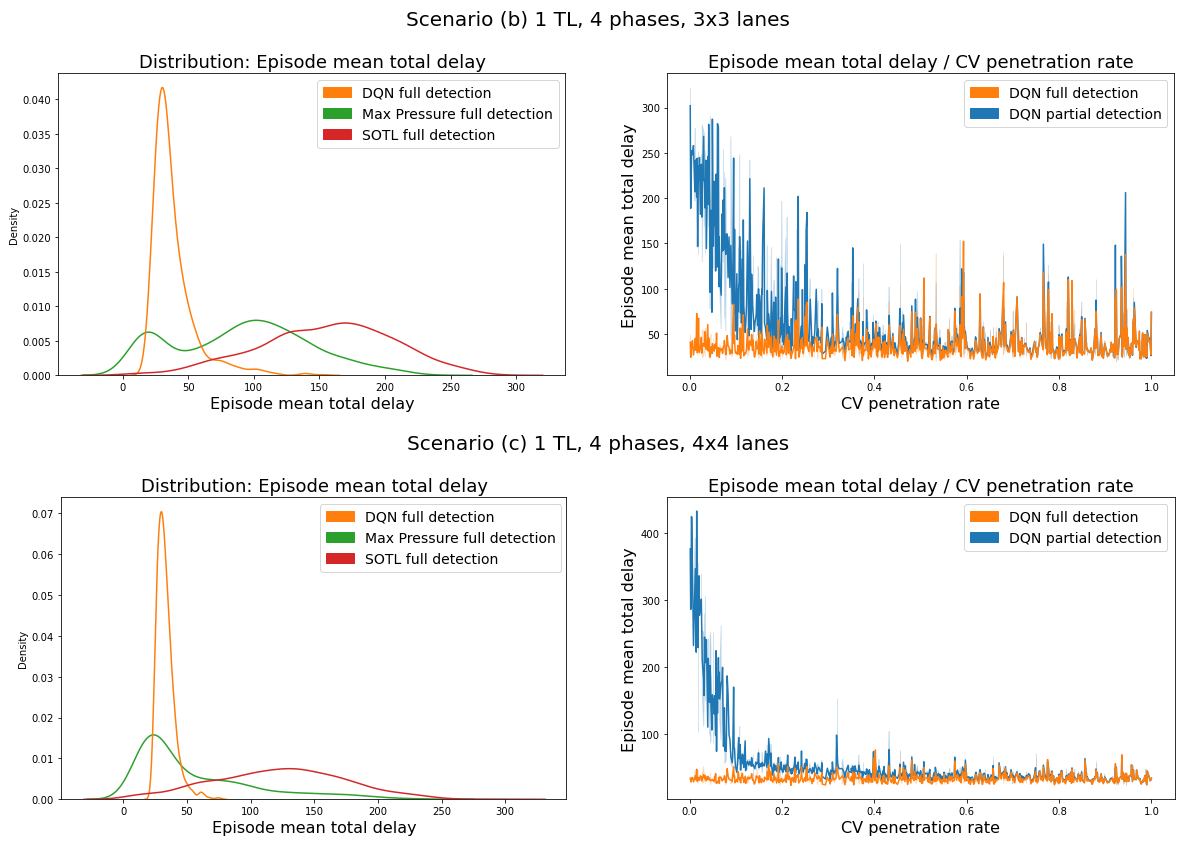
\includegraphics[width=\textwidth]{img/II/analysis_summary.png}
  \centering
  \captionsetup{justification=centering}
  \caption{Excerpts from figures (i) and (iii), for scenarios (b) and (c), and delay KPI.}
\end{figure}

\pagebreak

\subsubsection{Directions for future research}

\textbf{Discussion on limits and improvements} \\
We discuss hereinafter the identified current limits and points of further improvements: 
\begin{enumerate}
\setlength\itemsep{-0.5em}
  \item \textbf{Scenarios}: Here, only five scenarios were tested, all with 4-way intersections. The testing dataset could be diversified with more scenarios, with other network configurations, such as 3-way and 5-way intersections. Additionally, other unexplored road parameters could be included; e.g. prioritized vehicles, 8-phases TL programs, pedestrian crossings, level crossings, taxi services, bus stops, public transports, etc. 
  \item \textbf{Computing power}: Here, both training and testing were performed on an 8-core CPU in limited time. GPU computing could allow to augment the data and results; with (1) faster and longer training, on more difficult scenarios, and with better tuned hyper-parameters, for improved learned policies, and with (2) an expanded testing dataset, enriched both in quantity and quality, for added accuracy in the analysis.
  \item \textbf{Estimation}: Here, we formulated the assumption that information on connected vehicles are precisely known, noting however this statement to be questionable for CV positions due to imprecise infrastructures. Probabilistic estimation methods could be explored and applied to compensate for the uncertainty in measurements.
  \item \textbf{Observation}: Here, we trained a different agent for each new size of partial DTSE. Generalizing partial DTSE across multiple intersection sizes could reduce training time and stabilize performances. An option would be to train the agent on a larger intersection, and apply zero padding in the partial DTSE for smaller intersections.
  \item \textbf{Reward}: Here, we considered the total squared delay, a reward in a fully observable environment that does not allow for post deployment learning, i.e. outside the simulator. An agent with a reward based only on the partial detection of CVs could continue to learn and optimize its policy after being deployed at a real intersection.
  \item \textbf{Low $p_{cv} < 0.2$}: Here, we briefly proposed to handle very low CV penetration rates less than 20\% with a maximum green interval $T_{g,max}$, to simulate a cyclic pre-timed fixed program. This issue of degraded performances remains a major drawback and an obstacle towards usability, and a more efficient solution appears as a necessity.
  \item \textbf{Coordination}: Here, a single agent controls multiple TLs, without coordination and communication. While no significant interference was observed on scenarios (d) and (e), it would probably occur on larger networks. Thus, the model could be adapted to multi agent RL (MARL), for communicating grids of coordinated TLs.
  \item \textbf{Deployment}: Here, the model was deployed only on synthetic road networks in the Sumo simulator. It could be further deployed on real world networks in the simulator, such as the Luxembourg Sumo traffic (LuST) scenario, and, after sufficient validation and within the scope of a controlled experiment, at a real intersection.
\end{enumerate}

Overall, the results obtained before and the points of improvements raised above suggest the presented DQN-ITSCwPD model to be both promising and improvable in many ways. 

\pagebreak